\documentclass[border=15pt, multi, tikz]{standalone}
\usepackage{import}
\usepackage{ctex}% 中文支持
\usepackage{tikz}

\subimport{./}{init}
\usetikzlibrary{positioning}
\usetikzlibrary{3d} %for including external image
\usetikzlibrary{quotes,angles}
\usetikzlibrary{calc}
\usetikzlibrary{decorations.pathreplacing}

\def\DataColor{rgb:blue,5;white,5}
\def\ConvColor{rgb:yellow,5;red,2.5;white,5}
\def\ConvReluColor{rgb:yellow,5;red,5;white,5}
\def\PoolColor{rgb:red,1;black,0.3}
\def\PcColor{rgb:blue,5;red,2.5;white,5}
\def\PcSquashColor{rgb:blue,5;red,5;white,4}
\def\DcColor{rgb:blue,5;green,15}
\def\SumColor{rgb:blue,5;green,15}
% \def\SoftmaxColor{rgb:magenta,5;black,7}

\begin{document}
\begin{tikzpicture}

\tikzstyle{connection}=[ultra thick,every node/.style={sloped,allow upside down},draw=\edgecolor,opacity=0.7]

%%%%%%%%%%%%%%%%%%%%%%%%%%%%%%%%%%%%%%%%%%%%%%%%%%%%%%%%%%%%%%%%%%%%%%%%%%%%%%%%%%%%%%%%
%% ideas
%%%%%%%%%%%%%%%%%%%%%%%%%%%%%%%%%%%%%%%%%%%%%%%%%%%%%%%%%%%%%%%%%%%%%%%%%%%%%%%%%%%%%%%%
% state
\node[canvas is zy plane at x=0] (temp) at (0,0,0) {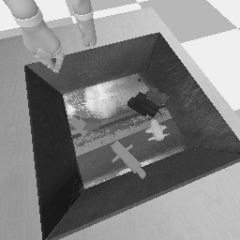
\includegraphics[width=6cm,height=6cm]{observation.png}};
\draw[connection] (1, 0, 0) -- node {\midarrow} (9, 0, 0);
% 注释
\node[] at (0, -4.5, 0) {机器人观察的图像状态};

\node[] at (5, 1, 0) {机器人依据观察执行一个动作};
% 下一个状态
\node[canvas is zy plane at x=0] (temp) at (10,0,0) {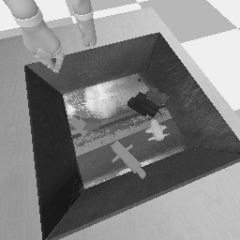
\includegraphics[width=6cm,height=6cm]{observation.png}};
% 
\node[] at (10, -4.5, 0) {机器人执行完动作后观察的图像状态};
%
\draw[connection] (10, 0, 0) -- node {\midarrow} (15, 0, 0);
% 注释
\node[] at (13, 1, 0) {机器人执行动作};
% 一步
\draw[decorate, decoration={brace, raise=15pt,amplitude=0.7cm},black!50] (10, -4.5, 0) -- (-1, -4.5, 0);
\node[] at (4.5, -6, 0) {一步};

% 中间过程
\node[canvas is xy plane at z=0] (temp) at (17,0,0) {
\includegraphics[width=4cm,height=4cm]{cellipsis.png}};

\draw[connection] (19, 0, 0) -- node {\midarrow} (23, 0, 0);
\node[] at (21, 1, 0) {机器人执行动作};

% 下一个状态
\node[canvas is zy plane at x=0] (temp) at (24,0,0) {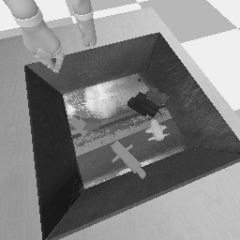
\includegraphics[width=6cm,height=6cm]{observation.png}};


\draw[decorate, decoration={brace, raise=15pt,amplitude=0.7cm},black!50] (25, -5.5, 0) -- (-1, -5.5, 0);
% 共有10步
\node[] at (12, -7, 0) {共有10步};




\end{tikzpicture}
\end{document}
